%
% File naaclhlt2010.tex
%
% Contact: nasmith@cs.cmu.edu

\documentclass[11pt,letterpaper]{article}
\usepackage{naaclhlt2010}
\usepackage{times}
\usepackage{latexsym}
\setlength\titlebox{6.5cm}    % Expanding the titlebox

\usepackage{amsmath}
\usepackage{graphicx}

\DeclareMathOperator*{\argmin}{arg\,min}
\DeclareMathOperator*{\argmax}{arg\,max}

\title{Social Dating: Matching and Clustering}

\author{
  SangHyeon (Alex) Ahn\\
  3900 North Charles St\\
  Baltimore, MD 21218, USA\\
  {\tt alexahn@jhu.edu}
  \And
  Jin Yong Shin\\
  3900 North Charles St\\
  Baltimore, MD 21218, USA\\
  {\tt jshin44@jhu.edu}
}
\date{}

\begin{document}
\maketitle
\begin{abstract}
Social dating is a stage of interpersonal relationship between two individuals for with the aim of each assessing the other's suitability as a partner in a more committed intimate relationship or marriage. Today, many individuals spend a lot of money, time, and effort for the search of their true partners. Some reasons for the inefficiency in seeking sexual partners include limited pool of candidates, lack of transparency in uncovering personalities, and the nature of time consumption in building relationships. Finding the right partner in a machine driven automated process can be beneficial towards increasing efficiency in the following aspects: reduced time and effort, a larger pool, and a level of quantitative/qualitative guarantees.

A binary classification prediction model predicting a potential match between a candidate and a partner can significantly improve social dating process in terms of increasing positive match outcomes. Also, clustering candidates who have similar demographic traits and preferences can help to narrow down the pool of potential partners for a given candidate.

In this paper, we modeled binary classification predictor for a potential match for a candidate, clustered candidates into similar demographic traits and preferences, and combined the two models for prediction model. In final stages, we have acquired a model with prediction accuracy near at 0.85.

\end{abstract}

\section{Introduction}
Purpose of the paper was to apply machine learning algorithms for Social Dating problems and build tools to be used for smarter decision making in matching process. We used the data from Speed Dating Experiment (of 21 waves) which includes each candidate's demographic attributes and preferences. We have selected relevant features to provide the most informative data and used $SQL$ to inner join missing feature variables.

We implemented Machine Learning algorithms (without the use of external libraries) to perform (1) binary classifications to predict a date match between a candidate and a potential partner, and (2) clustering analysis on candidates to use narrow down a pool of candidates by demographic traits and partner preferences. We have further combined the two model for acquiring a better prediction model. For our binary label, we gave $1$ as a match between two candidates and $-1$ as a non-match between the two.\\

We have constructed binary classification model using multiple algorithms each with varying parameters to select the best performing (highest prediction accuracy) model by tuning following parameters:
\begin{enumerate}
\item $I$: number of training iterations
\item $\theta$: regularization terms
\end{enumerate}

Also, clustering analysis is conducted under different $\lambda$ values for $\lambda$-means clustering to observe how many different clusters we may acquire from the data.\\

Each model's effectiveness and usefulness was also evaluated to verify suitability and validity, using accuracy testings and 5-fold cross-validation.

\section{Feature Engineering}

\subsection{Data}
Speed Dating Experiment data of 21 waves is provided by the research paper from University of Columbia conducting gender differences in mate selection, by Ray Fisman and Sheena Iyengar. The entire data has approximately ~5000 instances (4-minutes speed date instance) with ~150 different attributes including id, gender, match, age, race, candidate attributes, partner attributes, candidate preferences, partner preferences, interest ratings, shared interest correlations, income and so on.\\

For our model, we have selected only the relevant features for our train model. In addition to binary label indicating a $match$, There are five large feature categories in our selected features:

\begin{enumerate}
\item Candidate Demographic
\item Candidate Attributes \& Preference
\item Partner Demographic
\item Partner Attributes \& Preference
\item Interests \& Characteristics
\end{enumerate}

\textbf{Demographic} features include gender, age, race, field of study, income	range, career field.

\textbf{Attributes} include candidate's own measures of attractiveness, sincerity, humor, intelligence, and ambitiousness.

\textbf{Preferences} include the desirable attributes (dimensions are equal as above) of a potential partner as well as level of shared interests.

\textbf{Interests \& Characteristics} includes a correlation between two candidates' preferred interests and activities, importance of race, importance of religious background, frequency of dates, and frequency of going out.

\subsection{Refining and Sampling the data}

To create and collect the full data set with non-missing values and proper feature columns, we constructed a relational database in $SQL$ and performed inner join function to compile a full database as described above.\\

In order to perform analysis, we duplicated the database for two scenarios, one for classification using full data, and another for clustering analysis for a single candidate.\\

For both database, we performed 5-fold random sampling, then divided train data to test data, at size of $8:2$ ratio (training:8, testing:2) for cross validation.\\

\section{Algorithms}
We developed two different algorithms for (1) classification model (2) clustering analysis.

\begin{enumerate}
\item \textbf{Binary classification} models explored:

We explored three different classification models for our binary prediction model for predicting a candidate as a potential match for a person.

\begin{enumerate}
\item \textbf{\emph{Margin Perceptron}}\\
Perceptron is a mistake driven online learning algorithm that performs like a single neuron. Prediction label, $\hat{y_i}$, for an instance $x_i$ is computed as a sign value of the dot product between weight, $w$, and instance's feature vector.

\begin{equation}
\hat{y_i} = sign(w \cdot x_i)
\end{equation}

In the training algorithm, $w$ is updated whenever the classifier makes an incorrect prediction ($y \neq \hat{y}$), at each iteration in training stage. Margin Perceptron, however, updates $w$ whenever margin (dot product value) is not satisfied at a label prediction even when the prediction is correct, to ensure labeling with at least a margin.

\item \textbf{\emph{SVM (Pegasos)}}
Support Vector Machine is a linear classifier using max-margin principle.
SVM classifies data by constructing a hyperplane in high dimensional space that segregates data, while retaining max-margin between the hyperplane to each data points. The margin is enforced by the objective function solved by QP solver (or other optimization method described below).

\begin{equation}
f(w) = \min_w \lambda \frac{1}{2}||w||^2 + \frac{1}{N}\sum_{i=1}^N l(w;(x_i,y_i))
\end{equation}
\begin{equation}
l(w;(x_i,y_i)) = max{0, 1 - y<w,x>)}
\end{equation}
where $<\cdot, \cdot>$ refers to the inner product of two vectors. Here, bias term is omitted with the assumption that hyperplane crosses the origin.\\

Pegasos is a version of SVM refering to Primal Estimated sub-Gradient Solver, which takes a stochastic gradient descent to optimize the objective function stated above. Pegasos takes sub-gradient of $f(w;i)$ at iteration $i$, where learning rate continuously decreases at each iteration (function of time) to guarantee convergence. This algorithm adheres to online-training method with stochastic-optimization step rather than batch-optimization.\\

\item \textbf{\emph{K-Nearest Neighbors}}
\end{enumerate}
K-Nearest Neighbors algorithm is a classification method using labels of training instances to predict latent instance label by distances to the training instances (i.e. Euclidean distance).

K-Nearest Neighbors is an instance-based learning method which predicts a label by the labels of the nearest neighbors to the latent instance. 

\begin{align}
&\hat{y} = &\argmax_{y'} \sum_{i \in Xn} [y_i = y']
\end{align}
\\


\item \textbf{Clustering} analysis method explored:

Clustering is performed on all candidates who participated in the Speed Dating Experiment, to be able to group people into specific cluster which gathers people with similar demographic traits and partner preferences to each cluster. 

\begin{enumerate}
\item \textbf{\emph{$\lambda$-means}}\\
$\lambda$-means clustering is an unsupervised learning algorithm based on Expectation-Maximization algorithm, which is an iterative method of assigning expected cluster (by closest distance) for each instance then maximizing (expected) likelihood by updating the estimator (cluster mean) with maximum likelihood estimator at each iteration. $\lambda$-means clustering is a modified version of K-means clustering where $\lambda$ is used to formulate different number of clusters without a fixed number of clusters. Whenever distance is larger than $\lambda$, the algorithm creates another cluster to assign instances.

E-step:
\begin{align}
&k = &\argmin_{j} ||x_i - \mu^j|| \&\& ||x_i - \mu^j|| 
\end{align}

M-step:
\begin{align}
&\mu^k = \frac{\sum_{i=1}^n r_{ik} x_i}{\sum_{i=1}^n r_{ik}}
\end{align}

where $r_{ik}$ is an indicator having a value of $1$ is $i$th instance belongs to $k$th cluster and $0$ otherwise.
\end{enumerate}
\end{enumerate}

\section{Implementation and Method Results}

In this section, we discuss our methods and approaches used for selecting which binary classification model to predict potential match between a candidate and an opposing partner. Also, we give a detailed analysis on our reasoning behind choosing parameters for both classification model and clustering analysis.

\subsection{Binary Classification Model}

For choosing binary classification model, we conducted 5-fold cross validation on 3 different algorithms: (1) Margin Perceptron, (2) SVM (Pegasos) and (3) K-Nearest Neighbors.

%Plot of 5-folded cross validation for all 3 algorithms
\begin{figure}
  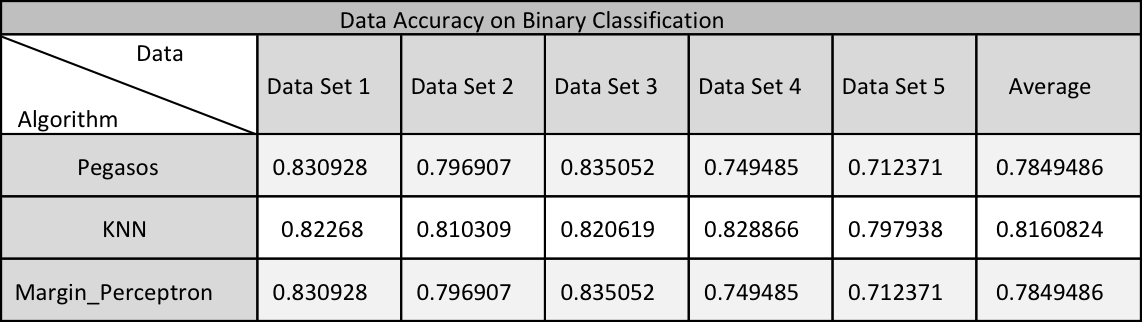
\includegraphics[width=\linewidth]{data_1.png}
  \caption{Binary Classification prediction accuracy using different algorithms}
  \label{fig:table1}
\end{figure}

\begin{figure}
  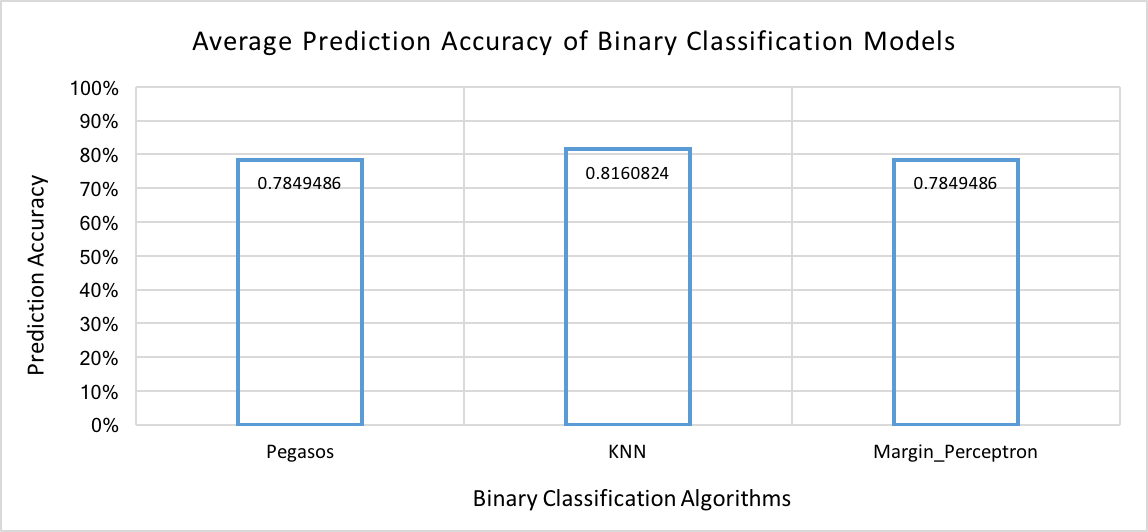
\includegraphics[width=\linewidth]{1_Raw_Binary_Classification.png}
  \caption{Binary Classification prediction accuracy using different algorithms}
  \label{fig:graph1}
\end{figure}

Figure \ref{fig:table1} and Figure \ref{fig:graph1} shows a changing behavior of prediction values by different algorithms for binary classifications using default parameters (training iterations=$10$, and $\$\theta=1.0$). Notice that $KNN$ performs best, then the other two models perform similarly.\\

Plot below show changes in prediction accuracy at different number of iterations.

%Plot iterations vs. accuracy for Pegasos & Margin Perceptron
\begin{figure}
  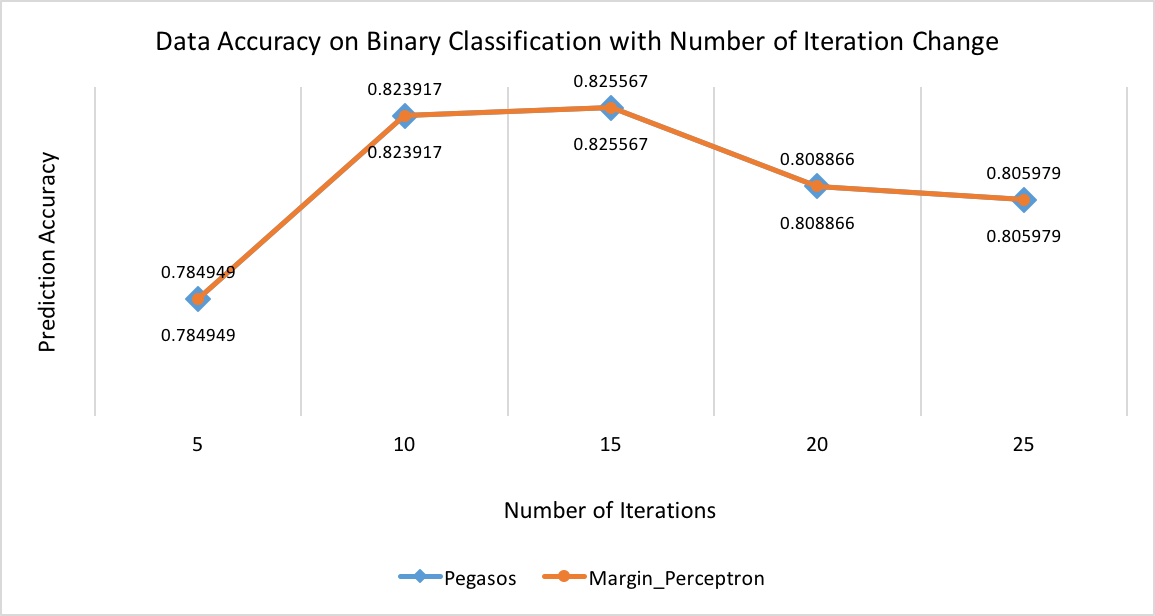
\includegraphics[width=\linewidth]{Normal_Prediction_Accuracy_with_Interation.png}
  \caption{Binary Classification at different iterations}
  \label{fig:table2}
\end{figure}

\pagebreak

\subsection{Clustering Analysis}

For clustering of candidates by demographic traits and preferences, we explored various values of $\lambda$ to observe data distribution behaviors.

%Plot lambda vs. # clusters
\begin{figure}
  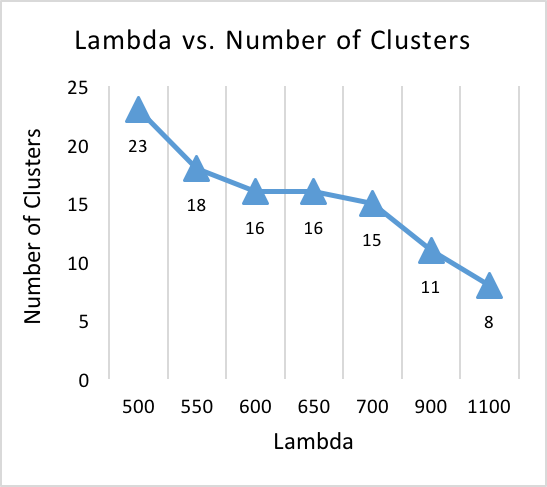
\includegraphics[width=\linewidth,height=6cm]{2_lamba_vs_cluster.png}
  \caption{Number of clusters at different $\lambda$}
  \label{fig:graph2}
\end{figure}

Figure \ref{fig:graph2} shows changes in number of clusters at different $\lambda$ values.

%Cluster numbers vs. VI
\begin{figure}
  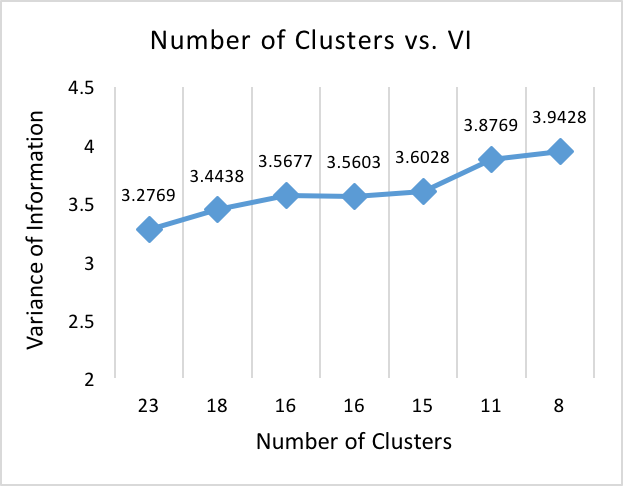
\includegraphics[width=\linewidth,height=6cm]{3_cluster_vs_VI.png}
  \caption{Variance of Information at different number of clusters}
  \label{fig:graph3}
\end{figure}

Figure \ref{fig:graph3} shows changes in Variance of Information (VI) at different cluster numbers.


%Plot Cluster numbers vs. accuracy
\begin{figure}
  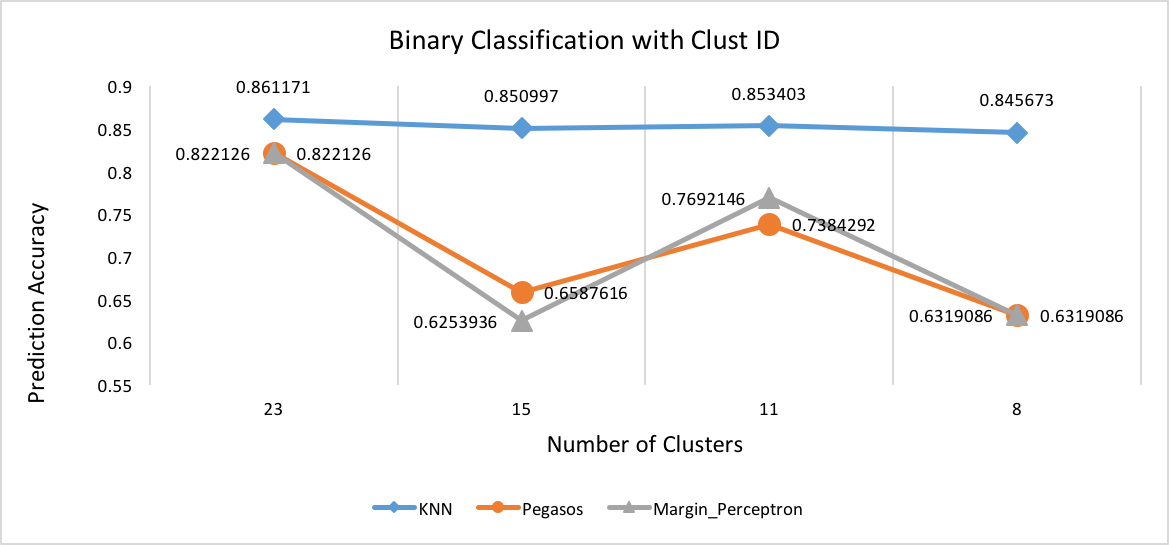
\includegraphics[width=\linewidth]{4_binary_classification_with_cluster_id.png}
  \caption{Variance of Information at different $\lambda$}
  \label{fig:graph4}
\end{figure}

Figure \ref{fig:graph4} shows changes in prediction accuracy for binary classification model using clusterID's as features, at different cluster numbers.

\pagebreak

\subsection{Combined Model}
Lastly, we combined the two models illustrated above to increase the performance of our prediction model. We have used the cluster assignments as a additive feature dimension in the classification model using three different algorithms.

%Plot of 5-folded cross validation
\begin{figure}
  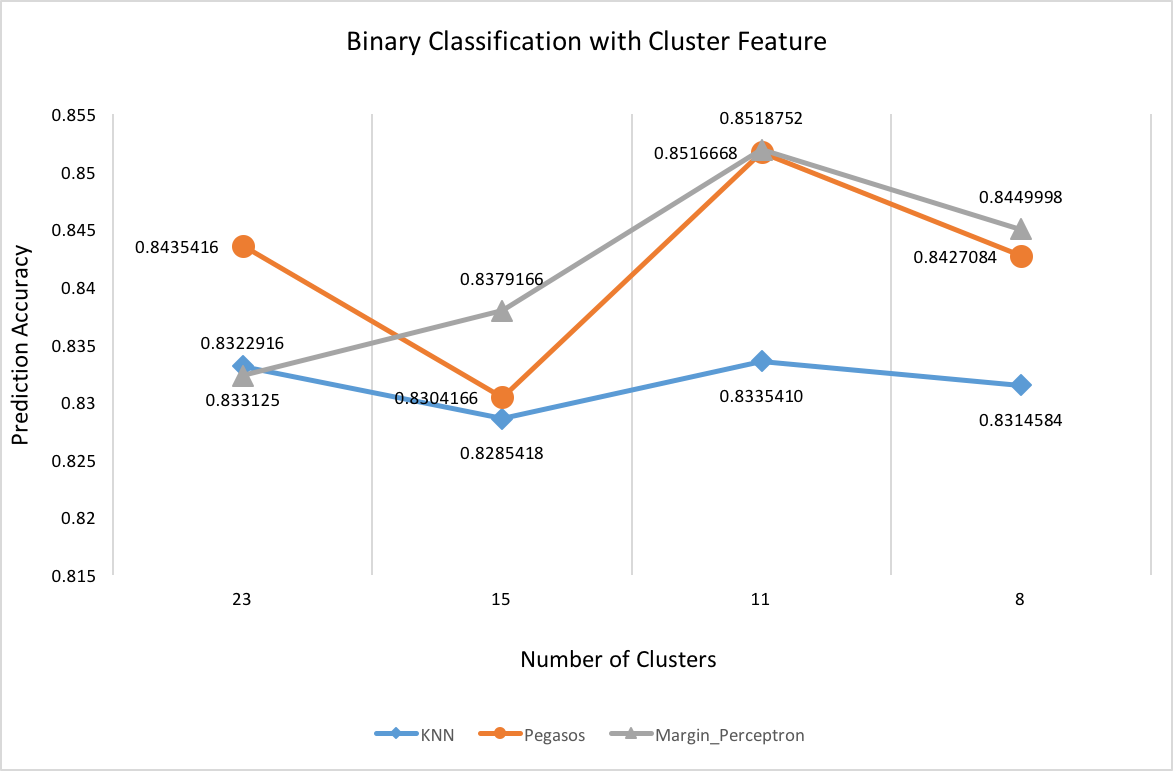
\includegraphics[width=\linewidth]{5_binary_classificatoin_with_clusdter_feature.png}
  \caption{Combined Model prediction accuracy with feature dimension with different number of clusters}
  \label{fig:graph5}
\end{figure}

The Figure \ref{fig:graph5} shows changes in prediction accuracy using different number of clusters as an additive feature dimension.

%Plot of 5-folded cross validation
\begin{figure}
  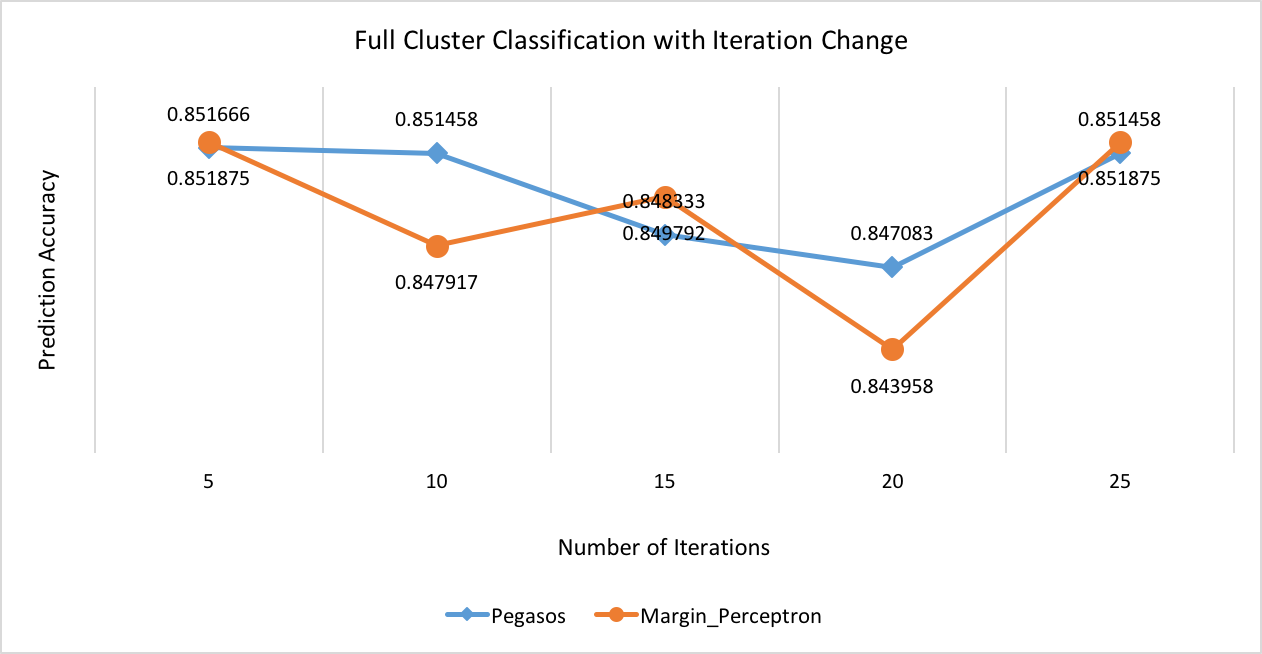
\includegraphics[width=\linewidth]{6_full_iteration_change.png}
  \caption{Combined Model prediction accuracy at different iteration numbers}
  \label{fig:graph6}
\end{figure}

The Figure \ref{fig:graph6} shows changes in prediction accuracy at different iteration numbers.

%Plot of 5-folded cross validation
\begin{figure}
  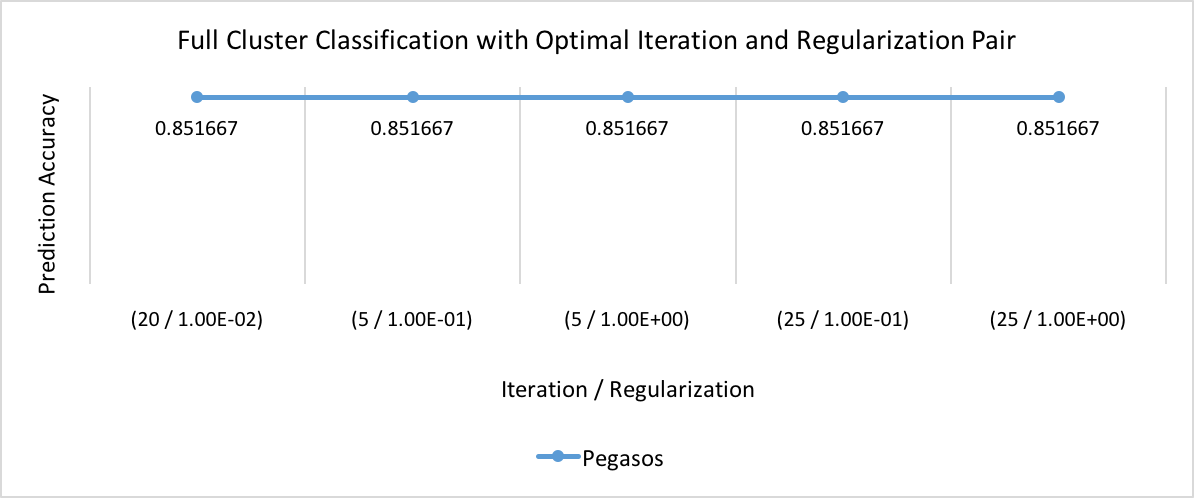
\includegraphics[width=\linewidth]{full_optimal_pair.png}
  \caption{Combined Model prediction accuracy at different iterations and regularization constant}
  \label{fig:graph7}
\end{figure}

The Figure \ref{fig:graph7} shows changes in prediction accuracy at different regularization constant.

\section{Evaluation and Model Selection}

As mentioned above, we performed 5-fold cross validation by randomly sampling the data into 5 different sets of train and test sets (8:2 ratio) to account for overfitting issues.\\

From the results presented above we can draw the following observations:

\begin{enumerate}
\item \textbf{Binary Classification Model}

At default parameter setting, resulting prediction accuracy is the following:
\begin{enumerate}
\item KNN: 0.816
\item Pegasos: 0.785
\item Margin Perceptron: 0.785
\end{enumerate}

We observe that KNN performs at best in terms of prediction accuracy, and that other two algorithms behaves similarly. However, we also observed that KNN runs at a much slower rate compared with the other two algorithms.

\item \textbf{Clustering Analysis}

We observe the following properties (VI and number of clusters) at different $\lambda$ values:

\begin{enumerate}
\item $\lambda=500$: 23 unique clusters / VI: 3.27
\item $\lambda=700$: 15 unique clusters / VI: 3.60
\item $\lambda=900$: 11 unique clusters / VI: 3.87
\item $\lambda=1100$: 8 unique clusters / VI: 3.94
\end{enumerate}

When using Cluster ID's as features for binary classification model we observe that KNN seems to perform best, however, this is due to the fact that there are only two features for calculating distances, and that there are a lot more labels for no match ($-1$) compared with match ($1$) that predicting as all non-match gives back good prediction accuracy.

\item \textbf{Combined Model}

In the combined model, we observe a noticeable contribution to prediction model with additive feature on dimension over cluster ID's.

We observe the following (best) prediction accuracy at each number of clusters, where Pegasos and Margin Perceptron outperform KNN:

\begin{enumerate}
\item 23 unique clusters : 0.844 (Pegasos) $|$ 0.832 (Margin Perceptron)
\item 15 unique clusters : 0.830 (Pegasos) $|$ 0.838 (Margin Perceptron)
\item 11 unique clusters : 0.852 (Pegasos) $|$ 0.852 (Margin Perceptron)
\item 8 unique clusters : 0.843 (Pegasos) $|$ 0.844 (Margin Perceptron)
\end{enumerate}

Generally speaking, both algorithms perform best when number of cluster equals $11$, which is at $\lambda=900$. In terms of algorithmic usage, Pegasos algorithm which is a version of SVM enables us to tune parameters including regularization terms while Margin Perceptron does not. Hence, Pegasos gives us a lot more flexibility which we can change the learning rate as well as regularization term to increase prediction accuracy in the future.\\

Therefore, from our experiment and observations, we chose Pegasos algorithm with Clustering analysis at $\lambda = 900$ that gives us feature dimension of $11$ different cluster ID assignments. Optimal number of iterations used for this algorithm was at $25$ iterations. Regularization factor did not seem to greatly affect the predictability. The resulting prediction accuracy is at $0.852$, for correctly predicting a match between a candidate and a potential partner.

\end{enumerate}

\section{Conclusion}

In conclusion, we have successfully modeled and chosen a prediction model using Pegasos Support Vector Machine (supervised binary classification algorithm) and $\lambda$-means clustering (unsupervised clustering algorithm), then we compiled a combined model using cluster ID's as features.\\

For tuning parameters we have chosen each by the results presented in section 4:

\begin{enumerate}
\item Pegasos: Iterations=$25$, Regularization($\theta$)=$1.0$
\item $\lambda$-means: $\lambda=900$
\item Combined Model: added feature dimension on cluster assignments by $\lambda$-means clustering
\end{enumerate}

Our final combined model gives us a prediction accuracy value of $0.852$ which we believe is a strong predictor.

\section*{Acknowledgments}

We thank professor Mark Dredze from Johns Hopkins University for supervising our project and helping us formulate the project idea using  machine learning algorithm.

\begin{thebibliography}{}

\bibitem[\protect\citename{Dredze}2016]{Dredze:1}
Mark Dredze.
\newblock 2016.
\newblock {\em Introduction to Machine Learning}
\newblock Baltimore, MD.

\bibitem[\protect\citename{Fisman and Iyengar}2016]{Fisman:1}
Ray Fisman and Sheena Iyengar.
\newblock 2005.
\newblock {\em GENDER DIFFERENCES IN MATE SELECTION:
EVIDENCE FROM A SPEED DATING EXPERIMENT*}
\newblock New York, NY.
\end{thebibliography}

\section*{Appendix}

\pagebreak

\vspace{1cm}

\begin{figure}
  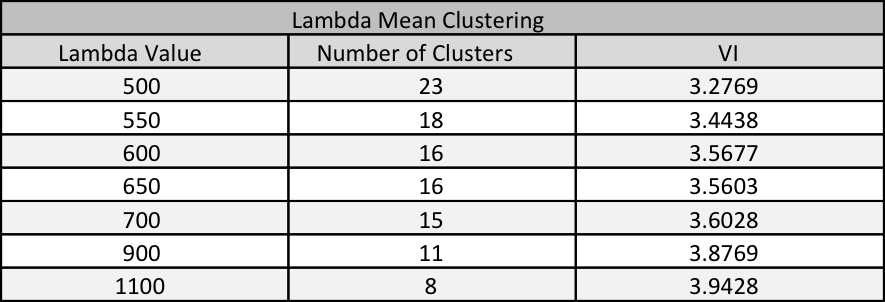
\includegraphics[width=\linewidth]{data_2.png}
  \label{fig:data_2}
\end{figure}

\begin{figure}
  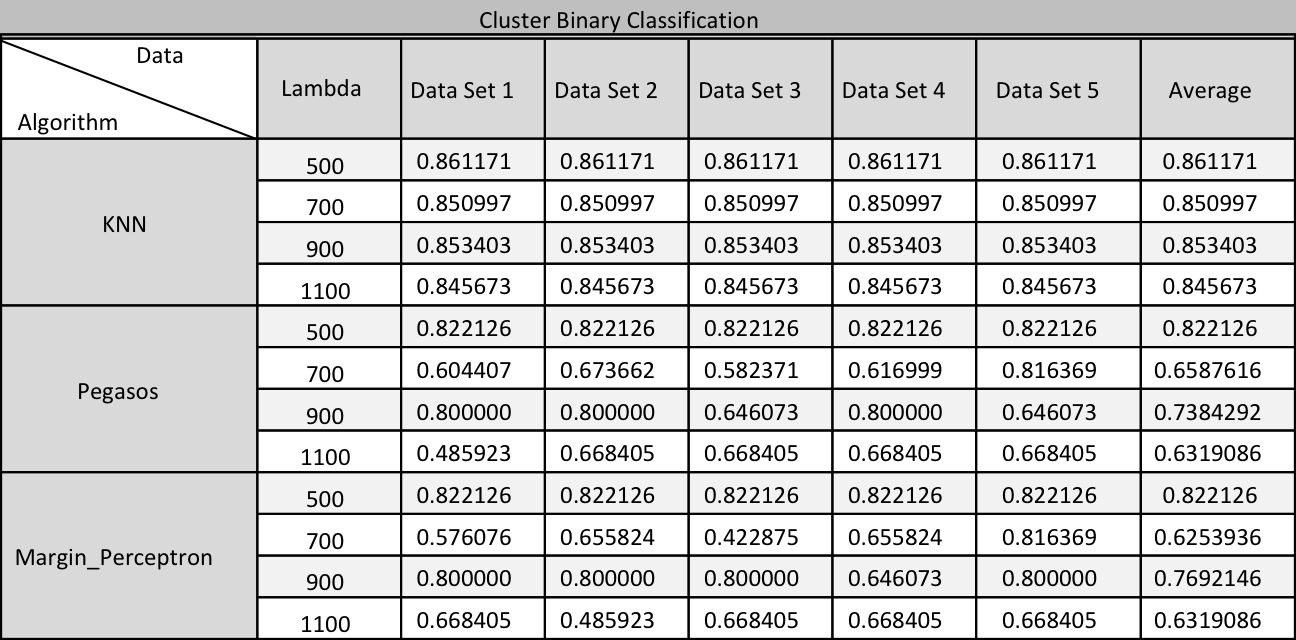
\includegraphics[width=\linewidth]{data_3.png}
  \label{fig:data_3}
\end{figure}

\begin{figure}
  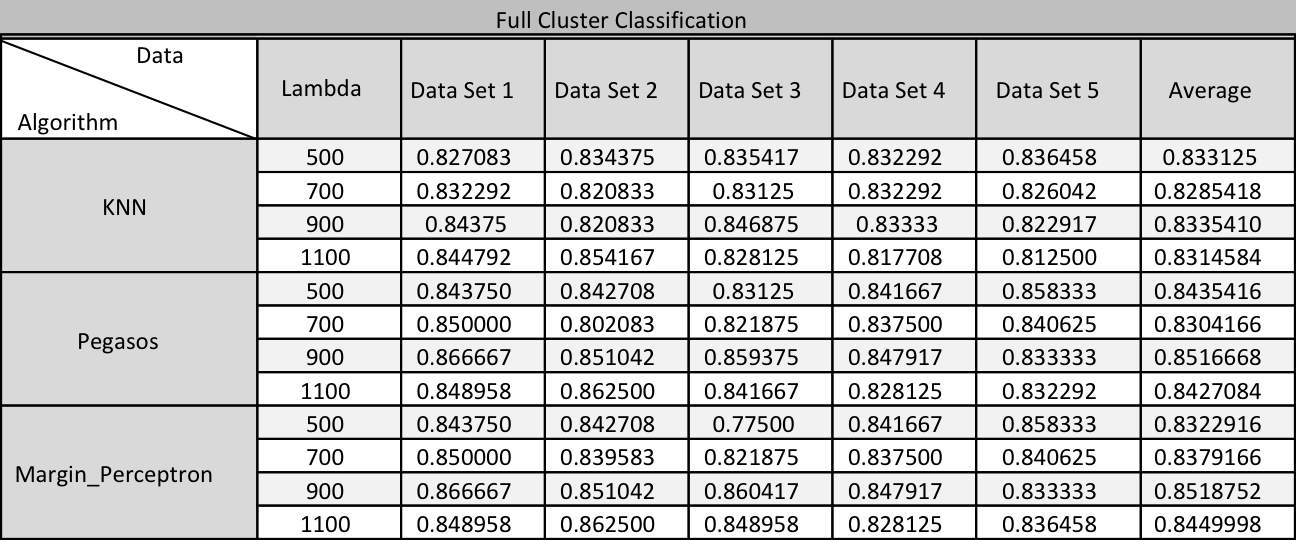
\includegraphics[width=\linewidth]{data_4.png}
  \label{fig:data_4}
\end{figure}

\begin{figure}
  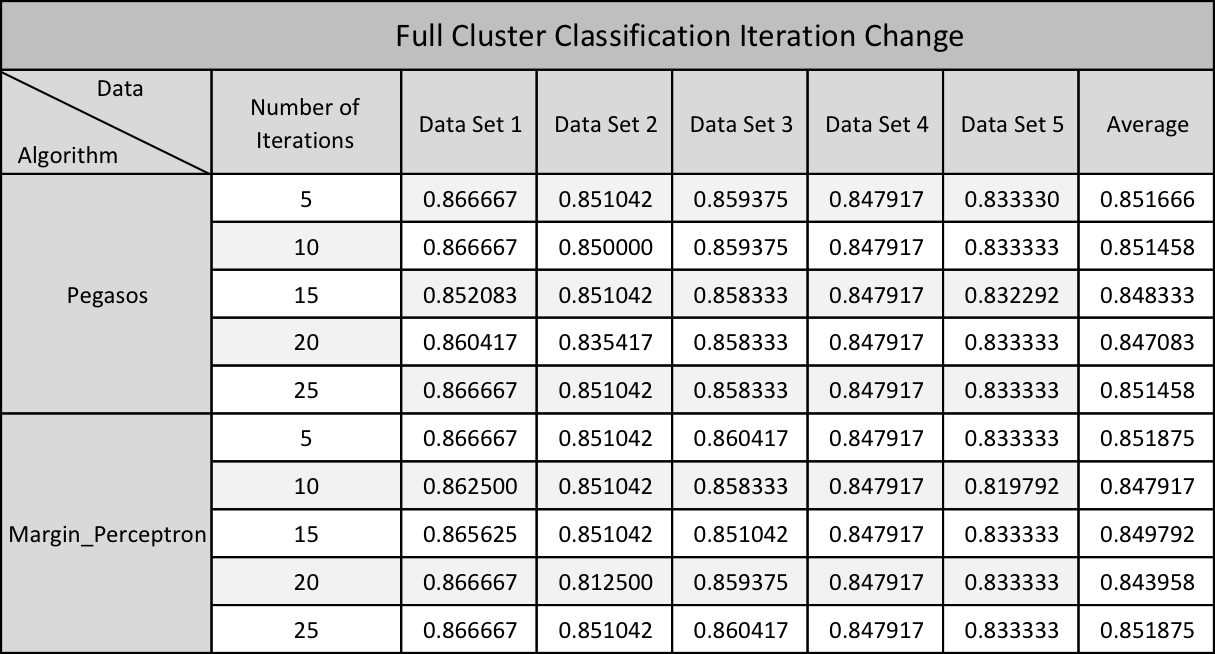
\includegraphics[width=\linewidth]{data_5.png}
  \label{fig:data_5}
\end{figure}

\begin{figure}
  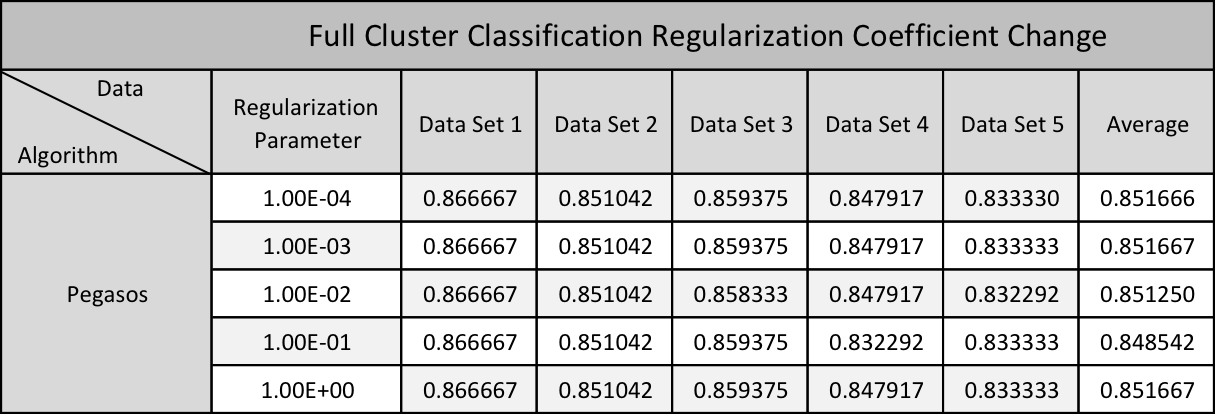
\includegraphics[width=\linewidth]{data_6.png}
  \label{fig:data_6}
\end{figure}

\begin{figure}
  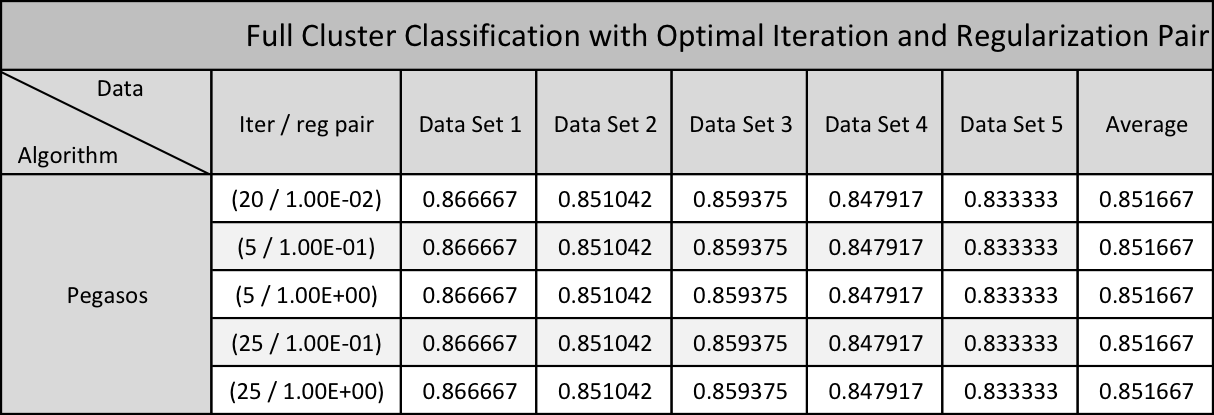
\includegraphics[width=\linewidth]{data_7.png}
  \label{fig:data_7}
\end{figure}

\begin{figure}
  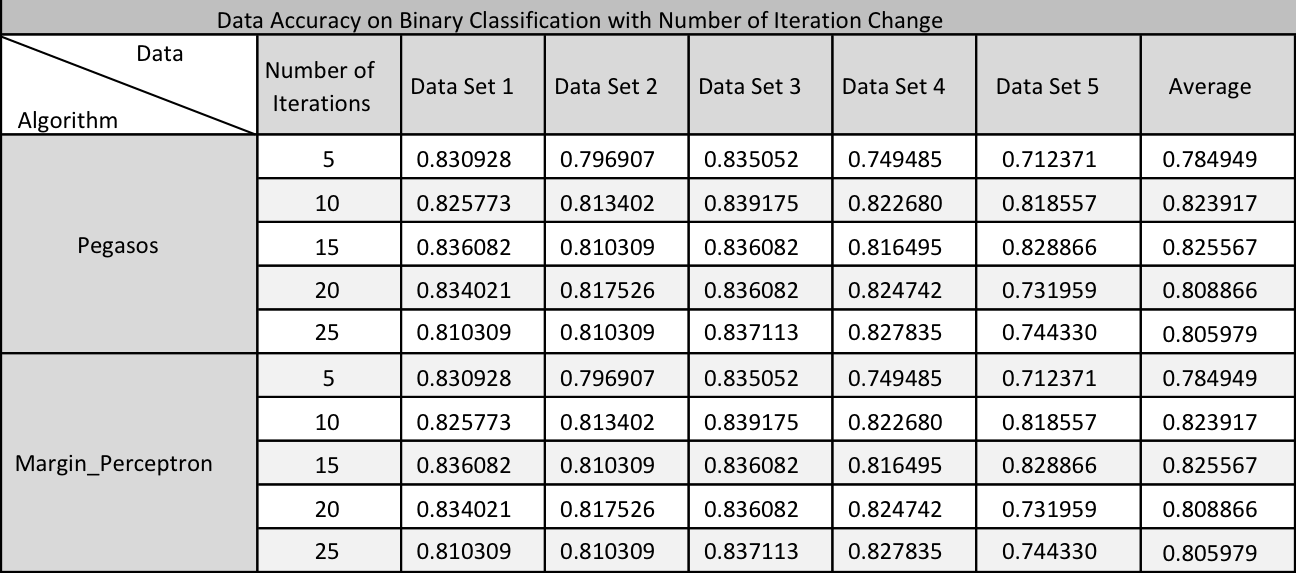
\includegraphics[width=\linewidth]{data_8.png}
  \label{fig:data_8}
\end{figure}


\end{document}
